%#####################################################################
\chapter{ネットワークモデルの動作検証}
%#####################################################################

 本研究は,ネットワークシミュレータであるns-3上でOpenFlowを用いたネットワークモデルを構築し,シミュレートすることで,ネットワークモデルが正常に動作するかを検証し評価することが目的である.
なお,今回の動作検証では実物のスーパーコアを使用せず,パケットが通過しただけで検査ができるというIPSの仕様を利用してIPS周辺でのパケットの流れを模したノードを作成し,そのノードの出力結果によってスーパーコアを通過したかを判定した.

シミュレーションでは,パケット通信を可視化するPyVizを用いての表示と,PCAPファイル形式でパケット内容を表示することが可能であるため,本章では,主にこの2つを用いて検証結果の評価を行った.

\section{ネットワークモデルの動作検証}

動作検証を行う際に,任意の2つのホストの位置関係に関する2つのケースを想定し,テストシナリオを作成した.

\begin{itemize}
	\item 送信元と送信先のコアスイッチの所属が違う場合
	\item 送信元と送信先のコアスイッチの所属が同じ場合
\end{itemize}

この2つのテストシナリオが正常に動作したならば,任意の2つのホスト間の通信は正常に動作したといえる.

この検証では,2つのホスト間でパケットを往復させるような通信を行わせる.
このときの通信プロトコルはUDPとし,シミュレーション時間の前半に往路の通信を,後半に復路の通信を行うようにした.

\subsection{送信元と送信先のコアスイッチの所属が違う場合}

送信元と送信先のコアスイッチの所属が違う場合の通信として,図 \ref{fig:4-1}のような通信経路が一例として挙げられる.
この例に従い,C++言語を用いてテストシナリオを作成し,シミュレータ上で実行した.

今回のテストシナリオでは,通信する2つのホストのIPアドレスを10.1.1.2と10.1.1.7とし,MACアドレスはIPアドレス10.1.1.7のホストの方が値が大きくなるように設定した.
そして,MACアドレスの大小関係を用いて経路選択を行うかを確認するために,MACアドレスの大きいホストを往路での送信元ホストとした.

\begin{figure}[tb]
	\begin{center}
		\scalebox{0.4}{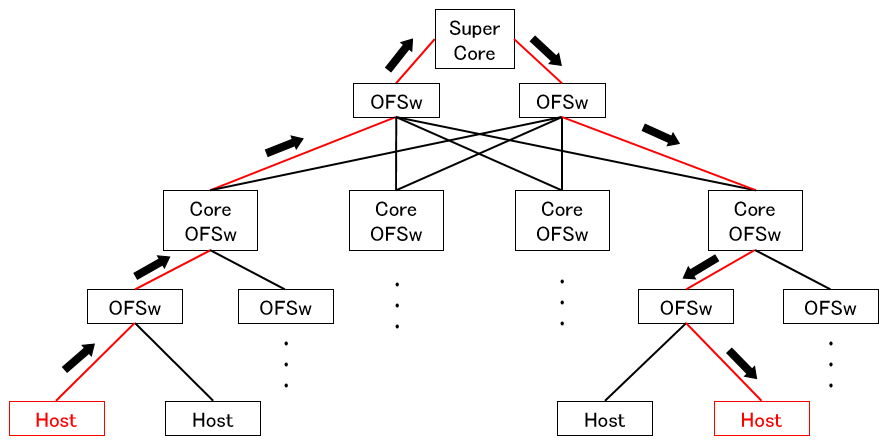
\includegraphics{./img/eps/4-1.eps}} 
		\caption{送信元と送信先のコアスイッチの所属が違う場合の例}
		\label{fig:4-1}
	\end{center}
\end{figure}

\begin{figure}[tb]
	\begin{center}
		\begin{tabular}{c}
			
			% 1
			\begin{minipage}{0.4\hsize}
				\begin{center}
					\scalebox{0.3}{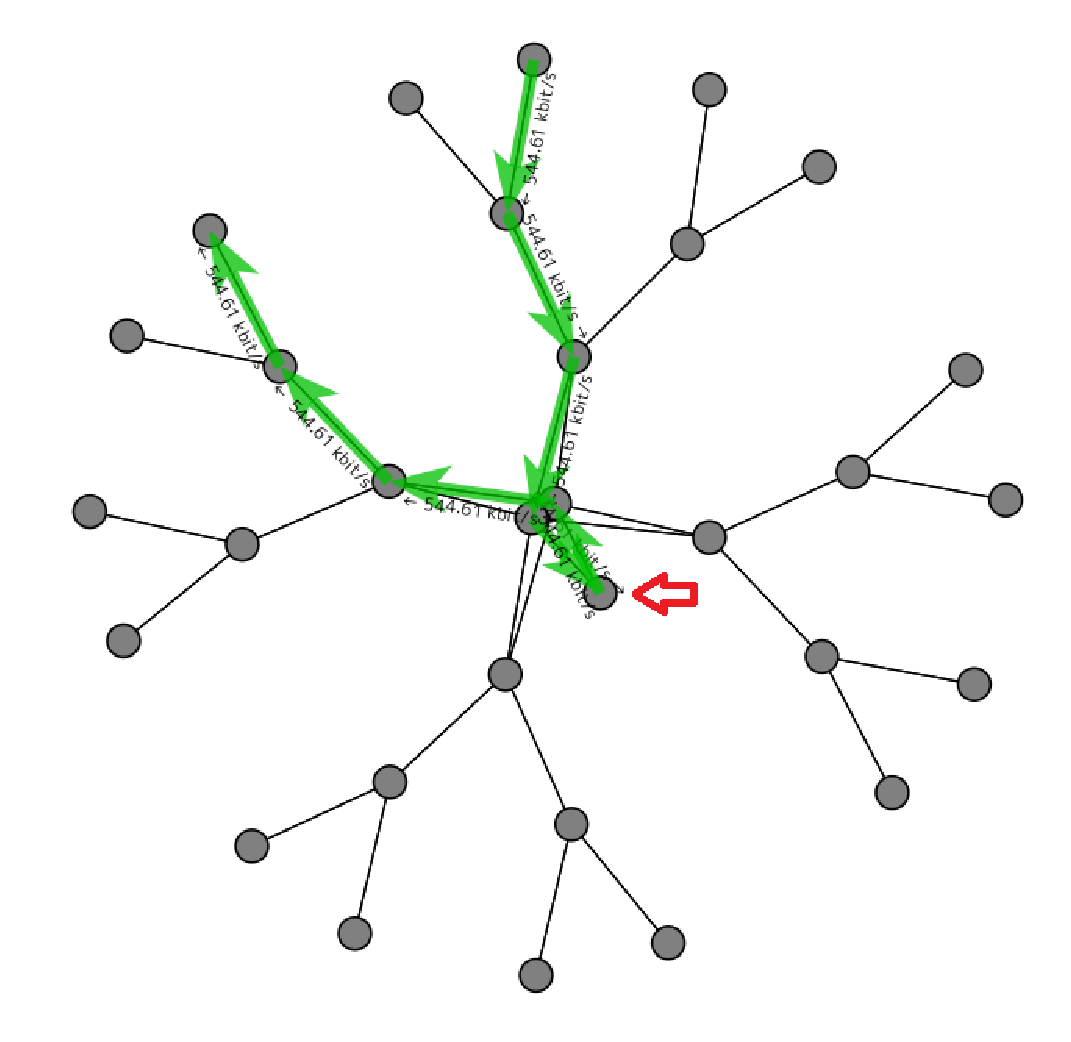
\includegraphics{./img/eps/4-2-1.eps}}
					\hspace{1.6cm} [1]往路の通信
				\end{center}
			\end{minipage}
			
			% 2
			\begin{minipage}{0.4\hsize}
				\begin{center}
					\scalebox{0.3}{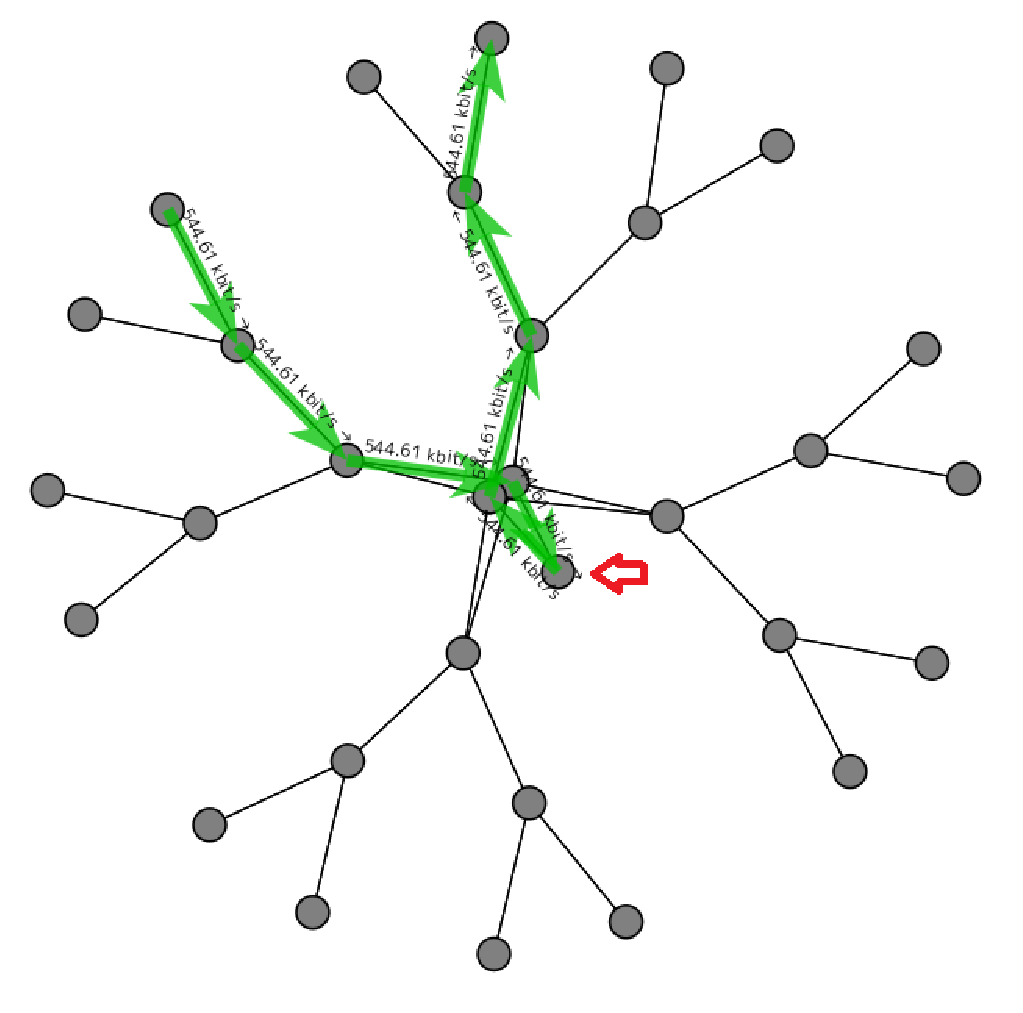
\includegraphics{./img/eps/4-2-2.eps}}
					\hspace{1.6cm} [2]復路の通信
				\end{center}
			\end{minipage}
			
		\end{tabular}
		\caption{送信元と送信先のコアスイッチの所属が違う場合の結果}
		\label{fig:4-2}
	\end{center}
\end{figure}

図 \ref{fig:4-2}は,テストシナリオを用いてシミュレーションした際のパケット通信を可視化したものである.
図 \ref{fig:4-2}内の赤の矢印で示したノードがIPSを想定したノードであり,往路の通信,復路の通信ともにパケットが正常にこのノードを経由して通信を行ったことが分かった.
更に,2枚の画像からホスト間の往復のパケットの経路が対称であることも確認できた.

\begin{figure}[tb]
	\begin{center}
		
		% 1
		\begin{center}
			\scalebox{0.8}{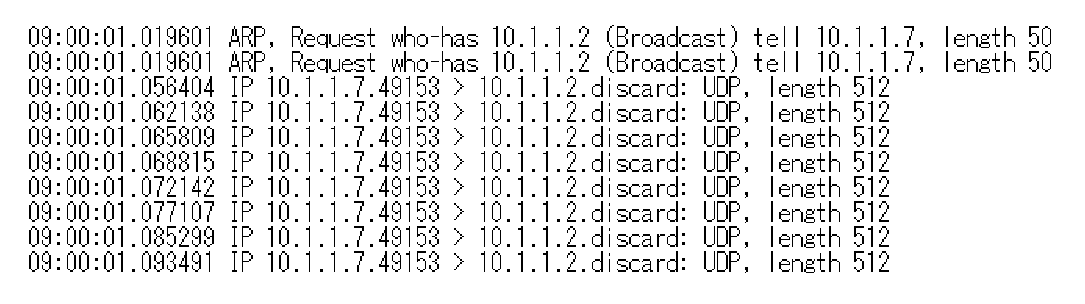
\includegraphics{./img/eps/4-3-1.eps}}
			\hspace{1.6cm} [1]往路の通信
		\end{center}
		
		% 2
		\begin{center}
			\scalebox{0.8}{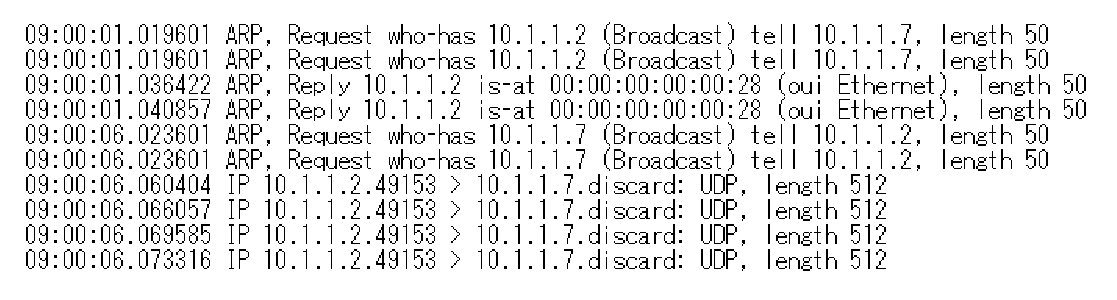
\includegraphics{./img/eps/4-3-2.eps}}
			\hspace{1.6cm} [2]復路の通信
		\end{center}
		\caption{送信元と送信先のコアスイッチの所属が違う場合のPCAPファイルの内容}
		\label{fig:4-3}
	\end{center}
\end{figure}

図 \ref{fig:4-3}は,IPSのそれぞれの物理ポートでのパケット出力を示すトレースファイルから,最初の10パケットの通過を切り取ったものである.
今回のシミュレーションでは,往路の通信は物理ポート0からの出力,復路の通信は物理ポート1からの出力であった.

トレースファイルによると,シミュレーションの前半にパケットを流した往路の通信が例外なく物理ポート0から出力され,物理ポート1からは,ARPを除くと後半にパケットを流す復路の通信が出力されていた.
つまり,送信元MACアドレスの値の方が大きくなるように設定した往路の通信では,スーパーコアを想定したノードに物理ポート1から入力したことを表し,復路の通信では,物理ポート0から入力されたことを表している.
このため,MACアドレスの比較によるスーパーコアの入力ポート決定の方法も正常に動作したといえる.

以上の内容からコアスイッチの所属が違う場合の通信は,全てスーパーコアを経由して通信されており,アルゴリズム通り正常に動作したといえる.

\subsection{送信元と送信先のコアスイッチの所属が同じ場合}

送信元と送信先のコアスイッチの所属が同じ場合の通信として,図 \ref{fig:4-4}のような通信経路が一例として挙げられる.
この例に従い,C++言語を用いてテストシナリオを作成し,シミュレータ上で実行した.

今回のテストシナリオでは,通信する2つのホストのIPアドレスを10.1.1.1と10.1.1.2とし,MACアドレスはIPアドレス10.1.1.2のホストの方が値が大きくなるように設定した.
また,MACアドレスの大小関係を用いて経路選択を行うかを確認するために,前節とは異なりMACアドレスの小さいホストを往路での送信元ホストとした.

\begin{figure}[tb]
	\begin{center}
		\scalebox{0.4}{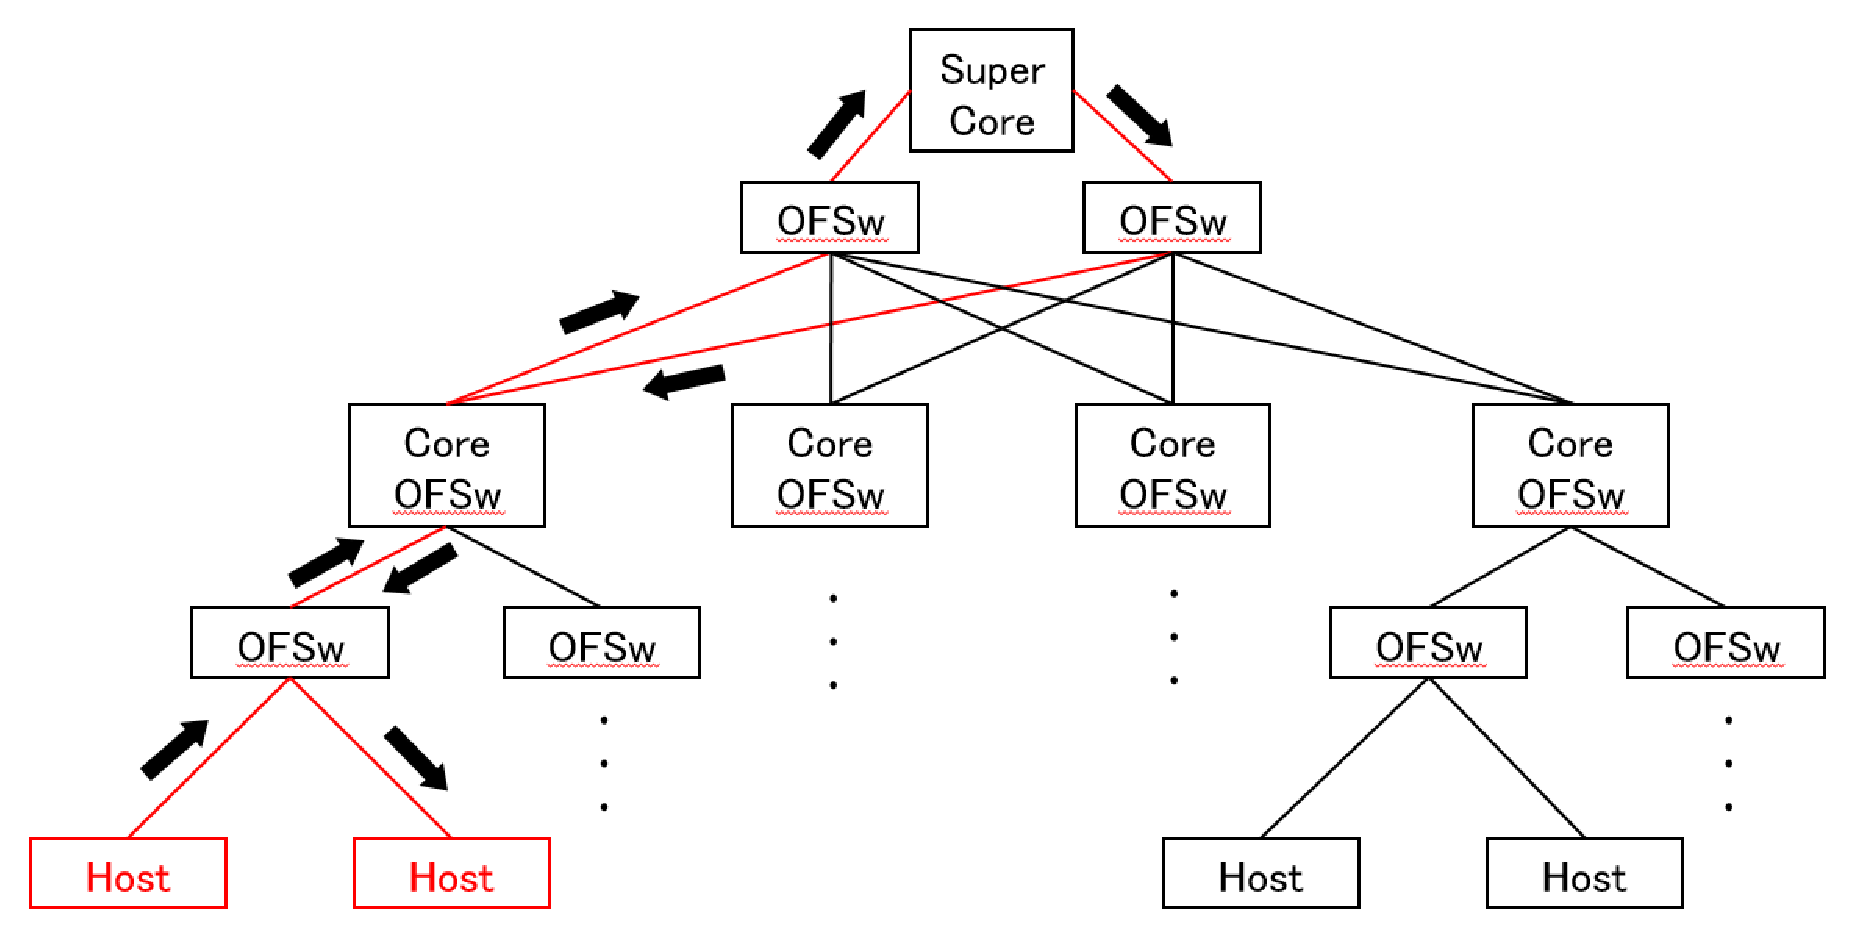
\includegraphics{./img/eps/4-4.eps}} 
		\caption{送信元と送信先のコアスイッチの所属が同じ場合の例}
		\label{fig:4-4}
	\end{center}
\end{figure}

\begin{figure}[tb]
	\begin{center}
		\begin{tabular}{c}
			
			% 1
			\begin{minipage}{0.4\hsize}
				\begin{center}
					\scalebox{0.3}{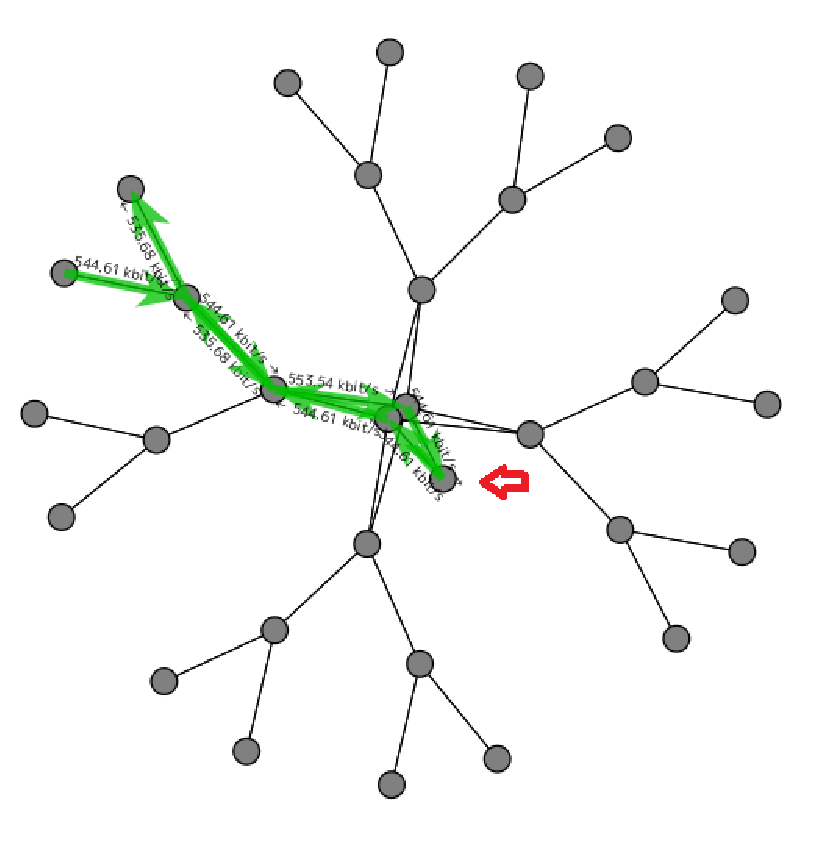
\includegraphics{./img/eps/4-5-1.eps}}
					\hspace{1.6cm} [1]往路の通信
				\end{center}
			\end{minipage}
			
			% 2
			\begin{minipage}{0.4\hsize}
				\begin{center}
					\scalebox{0.3}{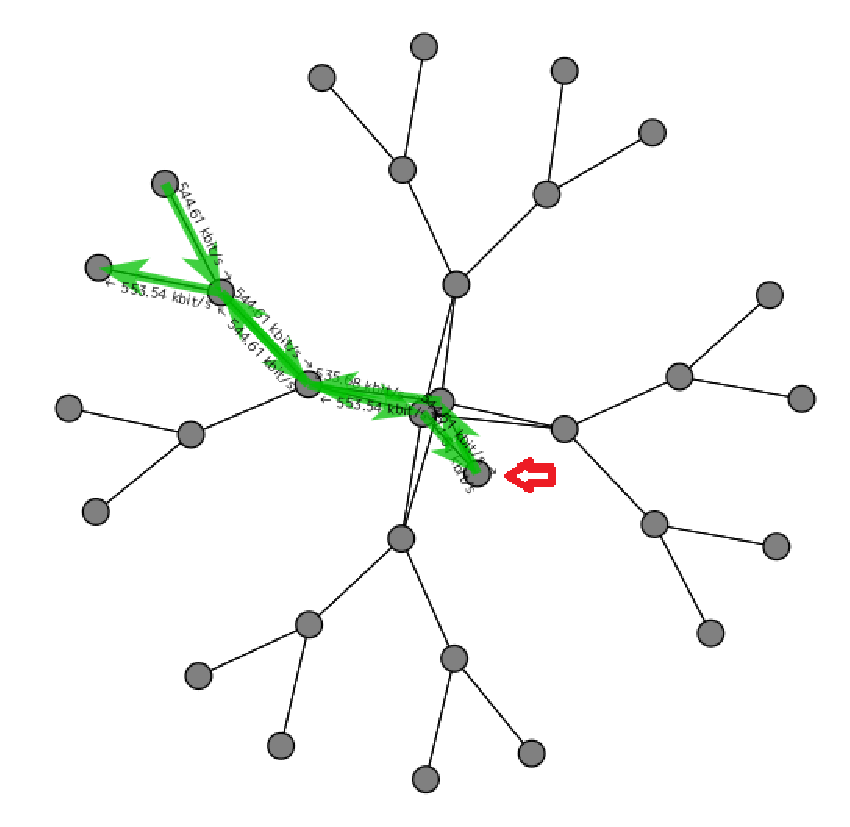
\includegraphics{./img/eps/4-5-2.eps}}
					\hspace{1.6cm} [2]復路の通信
				\end{center}
			\end{minipage}
			
		\end{tabular}
		\caption{送信元と送信先のコアスイッチの所属が同じ場合の結果}
		\label{fig:4-5}
	\end{center}
\end{figure}

図 \ref{fig:4-5}は,テストシナリオを用いてシミュレーションした際のパケット通信を可視化したものである.
図 \ref{fig:4-5}内の赤の矢印で示したノードがスーパーコアを想定したノードであり,往路の通信,復路の通信ともにパケットが正常にこのノードを経由して通信を行ったことが分かった.
これにより,スイッチがコントローラを無視して自律的に最短経路によって経路選択をせずに,コントローラに従って動作することもいえる.
更に,2枚の画像からホスト間の往復のパケットの経路が対称であることも確認できた.

\begin{figure}[tb]
	\begin{center}
		
		% 1
		\begin{center}
			\scalebox{0.8}{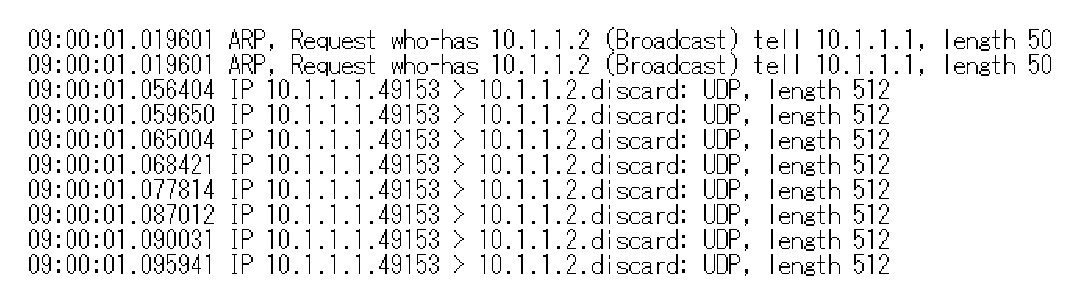
\includegraphics{./img/eps/4-6-1.eps}}
			\hspace{1.6cm} [1]往路の通信
		\end{center}
		
		% 2
		\begin{center}
			\scalebox{0.8}{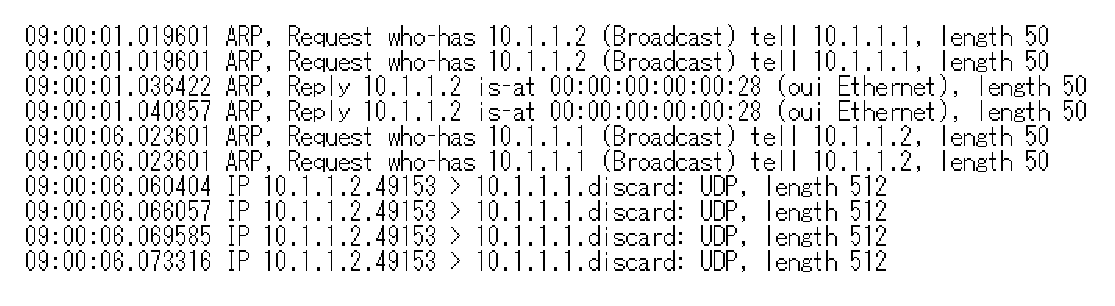
\includegraphics{./img/eps/4-6-2.eps}}
			\hspace{1.6cm} [2]復路の通信
		\end{center}
		\caption{送信元と送信先のコアスイッチの所属が同じ場合のPCAPファイルの内容}
		\label{fig:4-6}
	\end{center}
\end{figure}

図 \ref{fig:4-6}は,スーパーコアのそれぞれの物理ポートでのパケット出力を示すトレースファイルから,最初の10パケットの通過を切り取ったものである.
今回のシミュレーションでは,往路の通信は物理ポート1からの出力,復路の通信は物理ポート0からの出力であった.

トレースファイルによると,シミュレーションの前半にパケットを流した往路の通信が例外なく物理ポート1から出力され,物理ポート0からは,ARPを除くと後半にパケットを流す復路の通信が出力された.
つまり,送信元MACアドレスの値の方が小さくなるように設定した往路の通信では,スーパーコアを想定したノードに物理ポート0から入力したことを表し,復路の通信では,物理ポート1から入力されたことを表している.
このため,MACアドレスの比較によるスーパーコアの入力ポート決定の方法も正常に動作したといえる.

以上の内容からコアスイッチの所属が同じ場合の通信でも,スイッチがコントローラを無視して自律的に判断することはなく,全てスーパーコアを通して通信されており,アルゴリズム通り正常に動作したといえる.

% \section{MACアドレスの}